
\documentclass[12pt]{article}
\usepackage[letterpaper,textwidth=5.5in,right=0.6in,textheight=9in,left=0.6in,top=0.7in,bottom=0.7in]{geometry}

\usepackage{amsmath,amssymb}
\usepackage{graphicx}

\begin{document}
	\noindent Xinshi Wang\\
	661975305\\
	hw02\\
	
	\noindent 1.\\
	Claim: This graph does not have a cut-edge.\\
	We prove this by contradiction.\\
	Proof: Assume $\exists e \in E(G)$ such that $e$ is a cut-edge. Cut edge e will give us 2 separate components, $G_1$ and $G_2$. Since $\forall v \in V(G)$ we have $dv = 2k$(even) where $k \in \mathbb{N}$, $\exists v \in V(G)$ such that $d(v) = 2k+1$(odd) after cutting the edge e. Thus we have a vertex $v \in V(G_1)$ in one component with an odd degree, and the rest of the vertices in $G_1$ has even degrees. Thus the sum of degree in $G_1$ is an odd number. By the hand shaking theorem, $|E(G_1)|$ will not be an integer, which is impossible. Thus we have found a contradiction. Therefore such cut-edge $e$ does not exist.\\
	
	\noindent 2.\\
	The figure on the left is the graph generated using the graphic sequence, where the vertices are arranged in increasing order. The figure on the right is the tree generated using Prüfer code. \\
	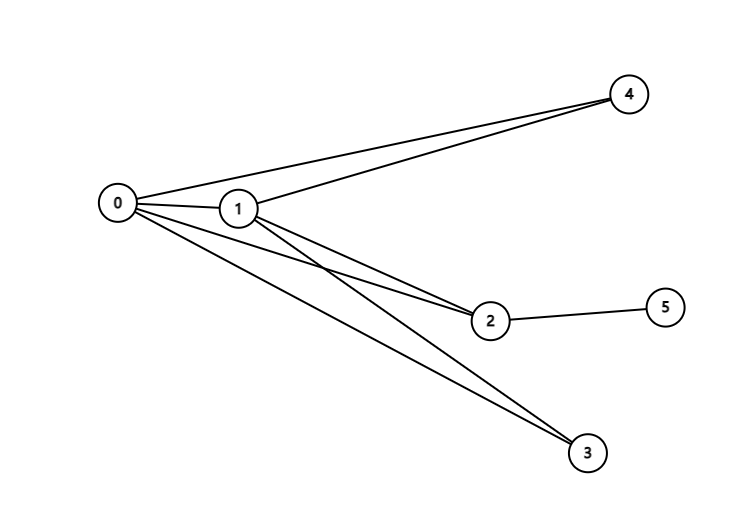
\includegraphics[scale = 0.4]{"C:/Users/Micha/OneDrive - Rensselaer Polytechnic Institute/Graph Theory/pictures/hw2-1.png"}
	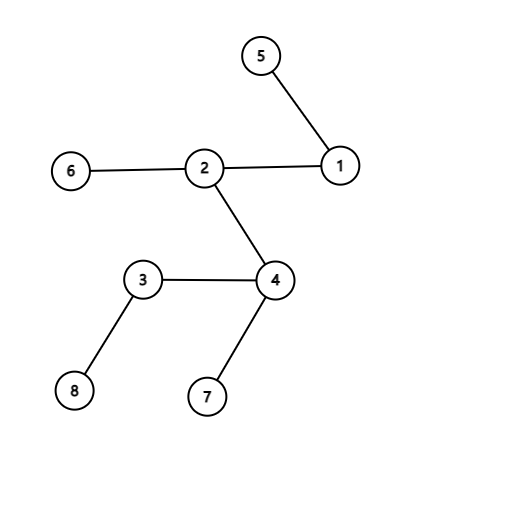
\includegraphics[scale = 0.4]{"C:/Users/Micha/OneDrive - Rensselaer Polytechnic Institute/Graph Theory/pictures/hw2-2.png"}\\
	
	\noindent 3.\\
	(a).Let $P(n)$ denote the statment that the number of leaves $l$
	on a tree $T$ with $|V(T)| = n$ is bounded below by the maximum degree of of the tree $k = \triangle(T)$.
	
	Base Case: $n = 1$. We have a graph with 1 vertex. This is trivial. $n=2$, we have a graph with two leaf vertices and an $edge$. $k < l$. $n = 3$. we have a graph with 2 leaf vertices and 2 edges.
	
	Inductive Step: Assume $p(1 \leq k' < n)$ holds, and prove $p(n)$ holds.
	
	Consider the case $k' = n-1$, and we have the tree $T'$. In order to prove $P(n)$ we need to add one vertex $u$ to $T'$. We could only add a leaf since adding a non-leaf edge creats a cycle, which violates the tree's property. Assume the vertex $v \in V(T')$ has the largest degree. We consider two exhaustive cases:
	
	1. $u$ is connected with $v$. In this case, the number of leaf vertices and the maximum degree both increased by one. Thus $k = k+1 \land l = l+1$. Since $l \geq k$ from our inductive hypothesis, $l+1 \geq k+1$. Thus in this case $P(n)$ holds.
	
	2. $u$ is not connected with $v$. In this case, the number of leaf vertices is increased by one and the maximum degree stays the same. Thus $k = k \land l = l+1$. Since $l \geq k$ from our inductive hypothesis, $l+1 \geq k$. Thus in this case $P(n)$ holds.
	
	Therefore P(n) holds in all cases, which means the number of leaves
	on a tree $T$ with $|V(T)| = n$ is bounded below by the maximum degree of of the tree.\\
	
	\newpage
	
	\noindent (b). Let us denote the vertex with the largest degree $v \in V(G)$. Vertex $v$ has $k$ edges, which implies there are $k$ unique paths since trees contains no cycle. The vertex that has the maximal $u-v$ path with vertex $v$ is a leaf node, other wise the path could be extended and the path would not be maximal. Thus the $k$ unique path will reach to at least $k$ leaf nodes, or more if one vertex on the path has degree greater than 2. Therefore $l \geq k$ and the number of leaves 
	on a tree $T$ with $|V(T)| = n$ is bounded below by the maximum degree of of the tree.\\
	
	\noindent (c). From the handshake theorem, we know $\sum_{v \in V(G)} deg(v) = 2|E| $. From the properties of trees, we know $|E| = |V|-1$. For the non-leaf vertices, the degree of each vertex is at least two to stay connected. Let $u$ denote the vertex with maximal degree in $G$, and let l denote the cardinality of the set of leaf vertices. Let leaf be the set of leaf vertices. Then we have the following formula.
	\begin{align*}
		\sum_{v \in V(G)} deg(v) &\geq deg(u) + \sum_{v \in V(G) \setminus L \cup \{u\}} deg(v)+ \sum_{v \in leaf} deg(v) \\
		 2(|E|) &\geq k + 2(|V|-|leaf|-1) + |leaf|\\
		 2(|V|-1) &\geq k + 2|V| - 2l -2 + l\\
		 l &\geq k 
	\end{align*}
	Therefore $l \geq k$ and the number of leaves 
	on a tree $T$ with $|V(T)| = n$ is bounded below by the maximum degree of of the tree.\\
	
	\noindent 4. 
	
	We prove case one by contradiction. Assume $|V(B_1)| \geq |V(B_2)|$ and there does not exist a leaf vertex in $B_1$, which means $\nexists v_1 \in V(B_1)$ such that $deg(v_1) = 1$. Then $\forall v_1 \in V(B_1)$, $deg(v_1) \geq 2$. Therefore $\sum_{v_1 \in V(B_1)} deg(v_1) \geq 2|V(B_1)|$. Since $\forall v_1 \in V(B_1)$, $v_1$ is connected to $v_2 \in B_2 \setminus B_1$, $\sum_{v_2 \in V(B_2)} deg(v_2) = \sum_{v_1 \in V(B_1)} deg(v) \geq 2|V(B_1)|$. Thus we have $\sum_{v \in V(B_1) \cup V(B_2)} deg(v) \geq 4|V(B_1)|$. By the handshake theorem, there are $|E'| = 2|V(B_1)|$ edges. According to the properties of tree, $|E| = |V(B_1)|+|V(B_2)|-1$. $|E'|$ must equal to $|E|$ by the property of tree, which means
	\begin{align*}
		|V(B_1)|+|V(B_2)|-1 &=  2|V(B_1)|\\
		|V(B_1)| &= |V(B_2)|-1
	\end{align*}
	From our assumption, we know $|V(B_1)| \geq |V(B_2)|$. Therefore we have a contradiction. Then there must $\exists v_1 \in V(B_1)$ such that $deg(v_1) = 1$, which means there must exist a leaf vertex in $B_1$. When $|V(B_1)| = |V(B_2)|$, this holds for both components and thus each of them must contain a leaf node.
	
	\newpage
	
	\noindent 5. Since graph $G$ is connected, $|E(G)| \geq |V(G)|-1$. Because $|V(G)| > |E(G)|$, it could only be the case that $|E(G)| = |V(G)|-1$. Therefore $G$ is a tree. Assume the maximal length path $P_1 ,P_2 \subseteq G$ have no intersections and $|P_1| = |P_2| = k$. Let us denote the set $P_1 = \{u_1,...,u_k\}$ and the set $P_2 = \{v_1,...,v_k\}$. For $u_i \in P_1$ and $v_j \in P_2$, there exists a unique path $p_3 = \{q_1,...,q_n\}$ connecting $u_i$ and $v_j$. $\exists a \in p_3$ and $a \notin P_1 \cup P_2$ since by definition $P_1$ and $P_2$ are not connected. Thus we have the non-empty set $Q = \{v:v\in P_3 \setminus (P_1 \cup P_2)\}$. Let us denote the path in $P_1$ starting from the end vertex in $P_1$ and end with vertex $u_i$ with length greater than or equal to $\dfrac{k}{2}$ as $P_1'$. Like wise we have $P_2'$. Since $|P_1'|+|P_2'|+|Q| = \dfrac{k}{2}+\dfrac{k}{2} +|Q| \geq k$, we know $P_1$ and $P_2$ are not the longest path. Thus there's a contradiction and thus $P_1$ and $P_2$ must have common vertices.\\
	
	\noindent 6. 
	Let us draw the following graph
	
	The spanning trees for the first graph on the RHS are $11$ as we discussed in lecture 7. The spanning trees for the second graph on the RHS is the sum of the number of spanning trees for the following graphs.
	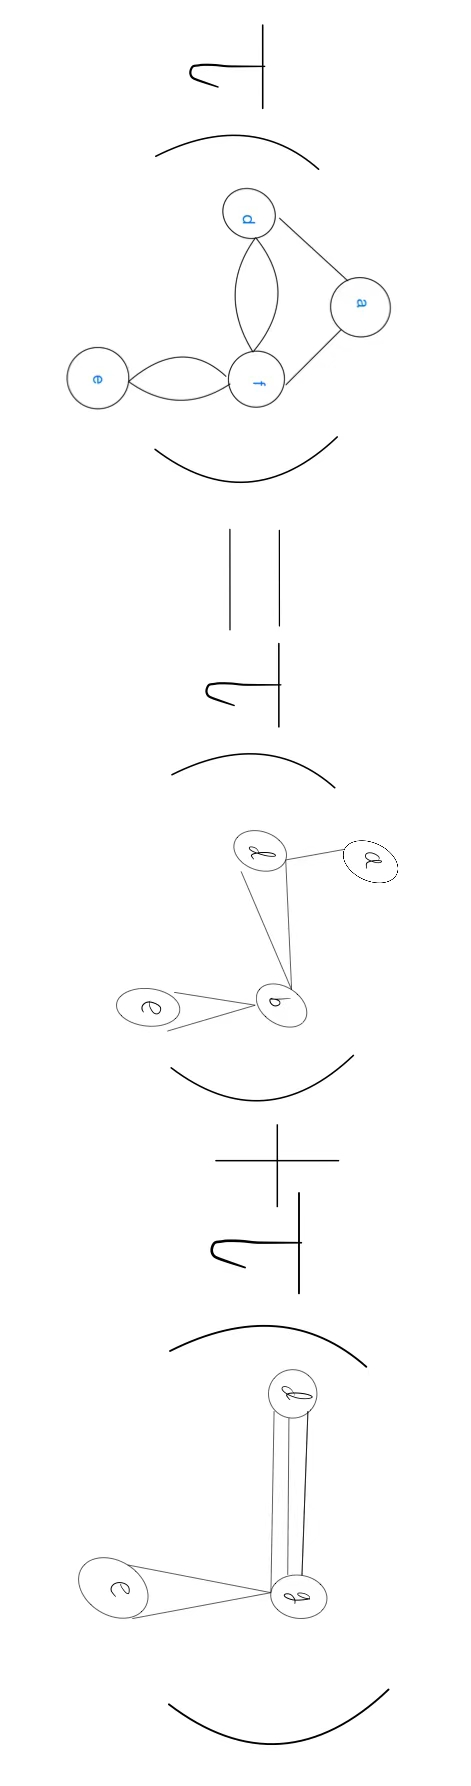
\includegraphics[scale = 0.42,angle=90]{"C:/Users/Micha/OneDrive - Rensselaer Polytechnic Institute/Graph Theory/pictures/hw2-6.jpg"}
	
	The number of spanning trees on the first graph on RHS is $2\times 2 = 4$ because there are two edges connecting $d$ and $b$ and two edges connecting $d$ and $e$. The number of spanning trees on the second graph on RHS is $3 \times 2 = 6$ because there are three edges connecting $d$ and $g$ and two edges connecting $g$ and $e$. 
	
	Thus there are in total $11+4+6 = 21$ spanning trees for the graph. 
	
	\noindent 7.
	
(a).\\

\begin{tabular}{lllllrr}
	$v\in G$ &       $E_1$ &       $E_2$ &       $E_3$ &       $E_4$ &  $E_5$ &  $E_6$ \\
	a &         0 &         0 &         0 &         0 &    0 &    0    \\
	b &         8 &         7 &         7 &         7 &    7 &    7     \\
	c &  $\infty$ &  $\infty$ &  $\infty$ &  $\infty$ &    8 &    8     \\
	d &         1 &         1 &         1 &         1 &    1 &    1     \\
	e &  $\infty$ &  $\infty$ &  $\infty$ &        12 &   10 &   10    \\
	f &  $\infty$ &         3 &         3 &         3 &    3 &    3     \\
	g &  $\infty$ &  $\infty$ &         6 &         6 &    6 &    6      \\
\end{tabular}
The order of processing order of verticies is $\{a,d,f,g,b,c,e\}$
(b).
We connect the smallest edges.

iteration 1: connect $ad$

iteration 2: connect $df$

iteration 3: connect $fg$

iteration 4: connect $gb$

iteration 5: connect $be$

iteration 6: connect $ec$

Thus we have the spanning tree $T = \{ad,df,fg,gb,be,ec\}$.
\end{document}